%
% Niniejszy plik stanowi przykład formatowania pracy magisterskiej na
% Wydziale MIM UW.  Szkielet użytych poleceń można wykorzystywać do
% woli, np. formatujac wlasna prace.
%   
% Zawartosc merytoryczna stanowi oryginalnosiagniecie
% naukowosciowe Marcina Wolinskiego.  Wszelkie prawa zastrzeżone.
%
% Copyright (c) 2001 by Marcin Woliński <M.Wolinski@gust.org.pl>
% Poprawki spowodowane zmianami przepisów - Marcin Szczuka, 1.10.2004
% Poprawki spowodowane zmianami przepisow i ujednolicenie 
% - Seweryn Karłowicz, 05.05.2006
% Dodanie wielu autorów i tłumaczenia na angielski - Kuba Pochrybniak, 29.11.2016

% dodaj opcję [licencjacka] dla pracy licencjackiej
% dodaj opcję [en] dla wersji angielskiej (mogą być obie: [licencjacka,en])
\documentclass[licencjacka,en]{pracamgr}

\usepackage{graphicx} %package to manage images
\usepackage{url}
\graphicspath{ {./images/} }
\usepackage[utf8]{inputenc}
\usepackage[rightcaption]{sidecap}
\usepackage{wrapfig}
\usepackage{titlesec}

\usepackage{listings}
\usepackage{xcolor}
\usepackage{float}

\definecolor{codegreen}{rgb}{0,0.6,0}
\definecolor{codegray}{rgb}{0.5,0.5,0.5}
\definecolor{codepurple}{rgb}{0.58,0,0.82}
\definecolor{backcolour}{rgb}{0.95,0.95,0.92}

\lstdefinestyle{mystyle}{
    backgroundcolor=\color{backcolour},   
    commentstyle=\color{codegreen},
    keywordstyle=\color{magenta},
    numberstyle=\tiny\color{codegray},
    stringstyle=\color{codepurple},
    basicstyle=\ttfamily\footnotesize,
    breakatwhitespace=false,         
    breaklines=true,                 
    captionpos=b,                    
    keepspaces=true,                 
    numbers=left,                    
    numbersep=5pt,                  
    showspaces=false,                
    showstringspaces=false,
    showtabs=false,                  
    tabsize=2
}

\lstset{style=mystyle}

% Dane magistranta:
% \autor{Adam Deryło, Adrian Hess, Magdalena Pałkus, Michał Skwarek}{34234234}

% Dane magistrantów:
\autor{Adam Deryło}{432952}
\autori{Adrian Hess}{431481}
\autorii{Magdalena Pałkus}{421537}
\autoriii{Michał Skwarek}{418426}
%\autoriv{Autor nr Cztery}{432145}
%\autorv{Autor nr Pięć}{342011}

\title{GPU acceleration of CCSDS Rice decoding}
\titlepl{Akceleracja GPU dekodowania CCSDS Rice}

%\tytulang{An implementation of a difference blabalizer based on the theory of $\sigma$ -- $\rho$ phetors}

%kierunek: 
% - matematyka, informacyka, ...
% - Mathematics, Computer Science, ...
\kierunek{Computer Science}

% informatyka - nie okreslamy zakresu (opcja zakomentowana)
% matematyka - zakres moze pozostac nieokreslony,
% a jesli ma byc okreslony dla pracy mgr,
% to przyjmuje jedna z wartosci:
% {metod matematycznych w finansach}
% {metod matematycznych w ubezpieczeniach}
% {matematyki stosowanej}
% {nauczania matematyki}
% Dla pracy licencjackiej mamy natomiast
% mozliwosc wpisania takiej wartosci zakresu:
% {Jednoczesnych Studiow Ekonomiczno--Matematycznych}

% \zakres{Tu wpisac, jesli trzeba, jedna z opcji podanych wyzej}

% Praca wykonana pod kierunkiem:
% (podać tytuł/stopień imię i nazwisko opiekuna
% Instytut
% ew. Wydział ew. Uczelnia (jeżeli nie MIM UW))
\opiekun{Paweł Gora\\
  Faculty of Mathematics, Informatics and Mechanics, University of Warsaw\\
  }

% miesiąc i~rok:
\date{Jan 2023}

%Podać dziedzinę wg klasyfikacji Socrates-Erasmus:
\dziedzina{ 
%11.0 Matematyka, Informatyka:\\ 
%11.1 Matematyka\\ 
% 11.2 Statystyka\\ 
11.3 Informatics, Computer Science \\ 
%11.3 Informatyka\\ 
%11.4 Sztuczna inteligencja\\ 
%11.5 Nauki aktuarialne\\
%11.9 Inne nauki matematyczne i informatyczne
}

%Klasyfikacja tematyczna wedlug AMS (matematyka) lub ACM (informatyka)
\klasyfikacja{D. Software\\
  D.1.3. Concurrent Programming\\
  I.4.2. Compression (Coding) \\ }

% Słowa kluczowe:
\keywords{CCSDS Rice coding, GPU, Compute Unified Device Architecture (CUDA)}

% Tu jest dobre miejsce na Twoje własne makra i~środowiska:
\newtheorem{defi}{Definicja}[section]

% koniec definicji

\begin{document}
\maketitle

%tu idzie streszczenie na strone poczatkowa
\begin{abstract}
\end{abstract}

\tableofcontents
%\listoffigures
%\listoftables

\chapter{Introduction}
\section{Background and motivation}
Machine learning (ML) has rapidly become a crucial tool for solving complex problems in a variety of domains, including computer vision, natural language processing, and speech recognition. However, ML pipelines can often experience significant bottlenecks due to multi-stage data processing pipelines that include loading, decoding, cropping, resizing, and other augmentations. This is particularly true when these processing steps are executed on a CPU, which is frequently the case. Since most of the machine learning training is already GPU accelerated due to ML workloads having a highly parallel nature, it is a natural progression to solve data processing bottlenecks by harnessing GPU acceleration. 

One such bottleneck is decompression of RICE-coded data, which is one of the most commonly used compression algorithms used in astronomy and astrophysics. Currently, there are only CPU-based solutions for decoding RICE-compressed data. It substantially hinders application of machine learning solutions in astronomy, especially considering the massive amount of training data already stored in RICE-compressed algorithm as well as being produced by observatories all around the world. To illustrate, just Solar Dynamics Observatory (SDO), with limited bandwidth due to being a satellite, is producing 130 megabits of RICE-coded data per second, that is 500 TB per year.

\section{Problem statement}
The problem at hand is that the current RICE decompression algorithm is computationally intensive and cannot keep up with the demand for high throughput and real-time processing. The goal of this project is to design and develop a GPU-based RICE decompression algorithm that can significantly accelerate the decompression process and improve the speed, efficiency, and scalability of ML pipelines in astronomy applications.

\section{Research objectives}
The main objectives of this thesis are as follows:

\begin{itemize}
    \item To study the existing literature on GPU acceleration of data compression and RICE decompression.
    \item To analyze the performance of RICE decompression on a CPU and a GPU.
    \item To design and implement a GPU-accelerated RICE decompression algorithm.
    \item To evaluate the performance of the GPU-accelerated RICE decompression algorithm and compare it with the CPU-based RICE decompression algorithm.
    \item And finally, to incorporate findings into NVIDIA Data Loading Library (DALI)\cite{dali-docs}, so machine learning, as well as the astronomy community, can utilize our findings.
\end{itemize}

\section{Thesis structure}
In this thesis, we present our attempts at parallelizing the RICE decompression algorithm and CUDA-based implementations of our findings. 

 Chapter 2 aims to define and explain key terms for our problem space, including the RICE algorithm itself. In the following chapter, we review previous work on the subject. We then present our solution architecture and how it ties into NVIDIA's open-source data-loading framework called DALI. Additionally, we introduce the Compute Unified Device Architecture (CUDA) to the reader. In Chapter 5, we propose a parallel implementation of the algorithm on GPU with details. Chapter 6 presents our performance and speedup results. Finally, in Chapter 7, we summarize our findings and conclude the thesis.

\chapter{Key terms}\label{r:pojecia}

\section{FITS format}

\subsection{Overview of FITS}

The Flexible Image Transport System (FITS) format is an openly documented digital file format commonly utilized in the field of astronomy for storing and transferring scientific data. The International Astronomical Union FITS Working Group (IAU-FWG) \cite{fits-working-group}is responsible for developing and maintaining the FITS format, with significant influence from the worldwide astronomy community. FITS format was designed for long-term usage, providing features such as backwards compatibility and standardization \cite{fits-standard}. FITS files typically contain images, data cubes, tables of observational data, and associated metadata, including observation date, instrument name, and coordinates.

One of the key characteristics of FITS is its ability to store multiple data arrays in a single file, enabling efficient storage and transfer of large datasets. FITS files are composed of the following structures in the listed order \cite{fits-official}:
\begin{itemize}
\item Primary HDU.
\item Conforming Extensions (optional).
\item Other special records (optional, restricted).
\end{itemize}

Thus, files usually resemble the following schema \cite{fits-image}:

\begin{figure}[h]
\centering
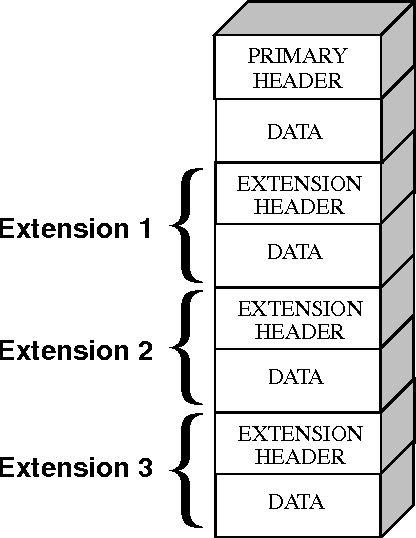
\includegraphics[scale=0.3]{fits}https://www.overleaf.com/project/637dd868a84cdd4898a13e23
\end{figure}

In every HDU including the primary one,  header contains relevant metadata as a list of key-value pairs. \cite{wikipedia} Furthermore, the most recent FITS standard published by CCSDS defines three types of standard extensions:
\begin{itemize}
\item IMAGE extensions.
\item TABLE ASCII-table extensions.
\item BINTABLE binary-table extensions.
\end{itemize}


\subsection{Compression of fits}

\subsubsection{Motivation}
In modern astronomy, observations produce huge datasets (even 12 TB per day \cite{crayondata} ) that are often archived and processed many years after their registration due to their size and quantity. Storing and managing data in compressed form is essential due to their smaller size. Compression of astronomical data is important for several reasons:
\begin{itemize}
\item Enabling storage of much more data in the same memory size.
\item Accelerating throughput between research centers.
\item Optimizing computational efficiency.
\item Following the strategy "Compress once, decompress never," many computational programs provide an interface to operate directly on FITS compressed files \cite{why-rice}. 
\item Many scientific tools are compatible and accept compressed FITS files.
\end{itemize}

\\

\subsubsection{Tile compression convention}

The tiled-image compression convention refers to the method of compressing images in the FITS format using a tiling approach. In this procedure, the FITS file is divided into smaller parts called tiles. Each tile is compressed independently, enabling efficient utilization of computational resources. This approach also allows for the decoding of specific parts of the data without having to decode the entire file. The CFITSIO library implements this convention and supports the following data compression algorithms: Rice, Hcompress, PLIO, and GZIP \cite{rice-comp}. Among these algorithms, the Rice algorithm is very efficient \cite{fpack} for compressing FITS files due to its higher speed and compression ratio compared to the others mentioned \cite{rice-comp}.

\subsubsection{Review of employed compression algorithms}

The most commonly used algorithms employing the tile compression convention are as follows \cite{rice-comp}:

\begin{itemize}
\item Rice: A simple and efficient lossless algorithm mentioned above.
\item Hcompress: A compression algorithm that uses wavelet transform followed by quantization and quadtree coding. By omitting the quantization step, Hcompress can also function as a lossless data compression algorithm.
\item PLIO (Piecewise Linear Image Compression with Optimization): An image compression algorithm that approximates an image using straight line segments.
\end{itemize}

\subsection{Benchmarks of various algorithms and why RICE was chosen}
The Rice compression algorithm is faster than alternatives like GZIP in terms of compression time for astronomical data (about 2-3 times faster) and results in a higher compression ratio of the input file by about 1.4 times \cite{rice-comp}. According to some papers, the Rice algorithm can also be faster in decompression \cite{why-rice}. These results indicate that using tile compression algorithms like Rice is more efficient for compressing astronomical data.

\section{CCSDS RICE coding}

\subsection{Golomb coding}
\subsubsection{History}
Golomb coding is losless data compression method named after its inventor, Solomon W. Golomb. It was first introduced in 1966. \cite{golomb-original}
\subsubsection{How it works}
In simple words, Golomb coding is a technique that is particularly effective for encoding non-negative integers. It uses a combination of unary and binary encoding to achieve efficient compression. In this procedure, index values $i$ are divided into equal groups of size $m$. \cite{golomb-coding-work} Next, the codeword are constructed from a unary code, that describe each group, followed by constant-size code $v_i$, that indicates the remainder of the index, that has been encoded.  Then, Golomb code residual is generated according to following formula \cite{golomb-coding-work}:
$$v_i = i - \left\lfloor\frac{i}{m}\right\rfloor \cdot m$$
\subsubsection{Pseudo Code}

\subsubsection{Example}

\subsection{Rice coding}
\subsubsection{History, how it is different from Golomb coding}
In RICE coding, invented by Robert F. Rice, that is subset of Golomb coding, using special $m$ values, according to formula: $m = 2^k$ \cite{golomb-coding-work}. This allows for the use of simple arithmetic bit-shifting operations that work in constant time, thereby accelerating the compression process.

The RICE algorithm is lossless, bit-wise data compression algorithm that uses a set of variable-length codes to compress data. As a lossless data compression algorithm \cite{rice-basics}, RICE is able to retrieve the full data from its compressed form without losing any part of the original data. The bit-wise algorithm operates on single bits (in contrast to byte-wise, which operates on single bytes), enabling greater compression due to the smaller granularity of the data they work with.

The essence of this algorithm is to use these codes to change symbols that are expected to be more frequent into shorter code words. The algorithm works on independently encoded data blocks, eliminating the need to transfer information between different packets. This improves performance and makes the RICE algorithm performance independent of data packet size \cite{rice-codes}.


\subsubsection{Pseudo Code}
Example of RICE encoding pseudo code is shown on following figure \cite{golomb-wikipedia}: \\
\begin{figure}[h]
\centering
\includegraphics[scale=0.5]{Rice_pseudocode}
\end{figure}

\subsubsection{Example}

\subsection{CCSDS RICE}
\subsubsection{How it differs from general implementation}
CCSDS RICE is a compression algorithm developed by the Consultative Committee for Space Data Systems (CCSDS) for space data applications. It is designed to achieve efficient compression while allowing reversible decompression, meaning the original data can be completely reconstructed from the compressed representation. CCSDS RICE uses a context selection mechanism to adaptively choose the optimal coding scheme for different data contexts.

CCSDS RICE operates by dividing the input data into blocks and encoding each block separately. It uses a combination of Golomb-Rice coding and Huffman coding techniques to encode the data efficiently. The Golomb-Rice coding is employed to handle the larger magnitude values, while Huffman coding is used for smaller magnitude values. The context selection mechanism helps determine which coding scheme is applied to each block based on the characteristics of the data.

For example, image encoding using the CCSDS RICE algorithm involves dividing the image into blocks of pixels and applying a predictive coding technique to compute and encode differences between the predicted value and the actual value. A variant of the Golomb coding is used, which uses a fixed-length prefix of binary zeros followed by a unary code to represent the quotient and remainder of the difference value \cite{rice-codes}. Unlike Golomb coding, where the number of bits needed to write the remainder depends on a variable parameter, the RICE algorithm uses data blocks of a constant size, resulting in a constant number of needed bits that is always a power of two. The prefix size typically depends on the characteristics of the image being compressed.

\subsubsection{Algorithm walk through}



The RICE algorithm consists of two main parts: a preprocessor and an adaptive entropy coder \cite{rice-basics}:
\begin{itemize}
\item The preprocessor is responsible for data processing before the actual compression. This part of the algorithm converts the input data into preprocessed samples and passes them to the Adaptive Entropy Coder.
\item The Adaptive Entropy Coder assigns shorter codes to symbols that occur more frequently and longer codes to symbols that occur less frequently. This part of the algorithm converts the preprocessed samples into the final encoded bit sequence.
\end{itemize}

\hfill \break
\hfill \break
\hfill \break
\hfill \break
This process can be ilustrated into following figure \cite{rice-basics}:
\hfill \break
\hfill \break
\centerline{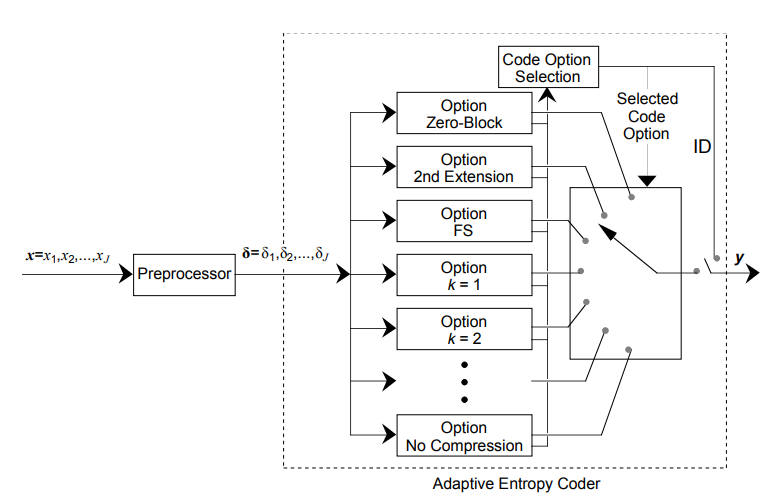
\includegraphics[scale=1.05]{RICE_encoder_architecture}}


% TODO:\\
% 1.Why compress at all? \\ 
% 2.Tile compression convention.\\
% 3.Review of employed compression algorithms. (and why rice is the best) \\ 

% Soruces: 
% https://heasarc.gsfc.nasa.gov/fitsio/fpack/O1.5.pdf  (1) 
% https://arxiv.org/pdf/0903.2140.pdf
% (2,3) 

\chapter{Related work}

\section{Overview of the problem space}
The acceleration of the Golomb-Rice algorithm has garnered significant attention in the literature, with most of the work focusing on the compression side of the problem. In particular, researchers have extensively studied Golomb parameter selection due to its critical role in determining achieved compression ratios. However, regarding throughput acceleration, the majority of the research has focused on implementing FPGA-based hardware acceleration for both compression and decompression. Notably, some software (CPU-based) approaches have been implemented, leveraging input format to achieve decoding throughput improvements from 1 Gbps to 4 Gbps \cite{fpga-dec}.

As for GPU-based acceleration, Xianyun Wu et al. evaluated the feasibility of GPU acceleration for the coding side of the issue in their study “Is the CCSDS Rice Coding Suitable for GPU Massively Parallel Implementation?” \cite{gpu-rice}. The authors achieved a six-fold speed up over the single-threaded CPU counterpart and concluded that CCSDS Rice coding contains numerous flow control instructions, significantly affecting the instruction throughput. These findings highlight the potential benefits of GPU-based acceleration for the coding side of the problem, but also suggest that further work is necessary to optimise CCSDS Rice coding for efficient GPU-based implementations.

\section{Current RICE decoding solutions in context of FITS}
To the best of our knowledge, the industry standard for compression and decompression of CCSDS Rice coded FITS files is achieved through the use of two standalone programs, fpack and funpack \cite{funpack-man}. These programs offer a unique advantage as they directly read and write the compressed FITS image format, eliminating the need for creating an uncompressed version of the file [why-rice](https://www.notion.so/why-rice-ab9d5ef4bfbd474bb049b8d3b0e047c2) . Additionally, fpack and funpack rely on the aforementioned tile compression convention and support multiple compression algorithms, including Hcompress, GZIP, and IRAF, apart from RICE \cite{funpack-user}. Both programs are included with CFITSIO\cite{funpack-man} , a FITS File Subroutine Library that is maintained by NASA’s High-Energy Astrophysics Science Archive Research Center (HEASARC) \cite{cfitsio}.

Regarding machine learning and data science workflows, where python is a prevailing programming language \cite{dev-survey}, either astropy or fitsio packages are mainly utilised \cite{astropy} \cite{fitsio} . While fitsio package is simply a Python wrapper for CFITSIO, astropy builds upon the PyFits package and is thus is a purely Pythonic implementation of various FITS File subroutines. Nevertheless, when it comes to compression, astropy accesses CFITSIO to support the FITS Tile Compression convention \cite{astropy}, what in the end makes them equivalent in terms of throughput in most cases. On that note, fitsio is shown to outperform astropy on the data sets consisting mainly of small files ($\sim0.3$ MB) \cite{astropy vs fitsio}, and thus it will be used for various Python-based benchmarks.

In summary, the fitsio and astropy packages offer convenient interfaces for accessing FITS files and decompressing CCSDS Rice encoded data in Python-based workflows. However, it should be noted that all of these packages rely on the same CPU-based RICE decompression algorithm implemented by funpack. While this algorithm has proven to be effective in achieving high compression ratios for a wide range of data types, it is limited in terms of its processing speed and throughput due to its CPU-based nature. As such, there is a growing interest in exploring alternative solutions that leverage emerging hardware technologies such as GPUs and FPGAs to accelerate the RICE decompression process. Such solutions have the potential to significantly improve the performance and efficiency of CCSDS Rice encoding and decoding in various domains, including machine learning, data science, and space science.

\chapter{Context}\label{r:losers}

\section{NVIDIA}
NVIDIA Corporation is a technology company known for designing and manufacturing graphics processing units (GPUs). Its professional line of GPUs are used in workstations for applications in such fields as architecture, engineering and construction, media and entertainment, automotive, scientific research, and manufacturing design. 

In addition to designing hardware, NVIDIA has made significant efforts to develop software tools and libraries that facilitate the use of their GPUs in scientific computing. Among these efforts, CUDA stands out as one of the most notable contributions. CUDA, which stands for Compute Unified Device Architecture, is a parallel computing platform and programming model that enables researchers to harness the power of GPUs for scientific computing tasks \cite{cuda-about}. With CUDA, developers can write programs in C, C++, and Fortran that can take advantage of the parallelism of GPUs to accelerate computations \cite{cuda-toolkit-official}. This has led to significant performance improvements for many scientific computing applications, including those in the fields of astrophysics, computational biology, and machine learning. 

To further support the use of GPUs in scientific computing, NVIDIA provides a range of software libraries that are optimised for use with CUDA. These include cuBLAS, cuFFT, and cuSPARSE, which provide high-performance implementations of common linear algebra, signal processing, and sparse matrix operations that are essential for many scientific computing applications\cite{nvidia-math-libs}. By offering these libraries, NVIDIA has made it easier for researchers and developers to take advantage of the power of GPUs in scientific computing.


%%\begin{itemize}
%\item {https://www.nvidia.com/en-us/about-nvidia/}
%\item {https://research.nvidia.com/publication/2021-12_evolution-graphics-processing-unit-gpu}
%\item https://www.nvidia.com/en-us/technologies/
%\item https://www.nvidia.com/en-us/data-center/ampere-architecture/
%\item https://developer.nvidia.com/cuda-zone
%\end{itemize}

\section{NVIDIA DALI}

The NVIDIA Data Loading Library (DALI) is a high-performance, portable, and open-source library for data loading and pre-processing in deep learning applications. It provides a collection of highly optimised building blocks for loading and processing image, video, and audio data. DALI can be used as a drop-in replacement for built-in data loaders and data iterators in popular deep learning frameworks, such as TensorFlow, PyTorch, and MXNet \cite{dali-docs}. \\
\\

\centerline{\includegraphics[scale=0.3]{images/dali.png}}

DALI addresses the problem of the CPU bottleneck by offloading data pre processing to the GPU. To do so DALI relies on its own execution engine, built to maximise the throughput of the input pipeline. This results in significant performance improvements for deep learning applications that require complex, multi-stage data processing pipelines \cite{blogpost}. 


\subsection{Core concepts}
In DALI, the central component is the data processing pipeline, which consists of a symbolic graph connecting data nodes through operators. These operators receive inputs, perform various data processing operations, and generate outputs. DALI categorises its operators into three types based on their backend: CPU, Mixed, and GPU. The CPU operators handle data on the CPU, while Mixed operators transfer data from the CPU to the GPU for processing, and GPU operators handle data entirely on the GPU. The pipeline itself is defined in Python in an imperative manner similarly to how object definition is implemented in other deep learning frameworks, such as Pytorch or Tensorflow. Nonetheless, after instantiation pipeline is actually executed under the hood by the code written in C++ which allows for more efficient asynchronous processing. \cite{blogpost}   Here is an example of pipeline definition: \\ 

\begin{lstlisting}[language=Python]
from nvidia.dali import pipeline_def, fn

@pipeline_def  
def my_pipeline():
    img_files, labels = fn.readers.file(file_root="image_dir", seed=1)
    mask_files, _ = fn.readers.file(file_root="mask_dir", seed=1)
    images = fn.decoders.image(img_files, device="mixed")
    masks  = fn.decoders.image(mask_files, device="mixed")
    return images, masks, labels

pipe = my_pipeline(batch_size=4, num_threads=2, device_id=0)
pipe.build()
\end{lstlisting}

Which  results in following data processing graph: \cite{dali-docs} \\

\centerline{\includegraphics[scale=0.5]{images/dali-flow.png}}

Among many other optimizations, such architecture allows for data prefetching, that is, preparing batches of data ahead of time before they are requested. This ensures that the framework always has data readily available for the next iteration. The purpose of data prefetching is twofold: firstly, it helps to mask the latency associated with preprocessing, which becomes particularly crucial when the processing time varies significantly across iterations. Secondly, it mitigates the bottleneck caused by input/output (IO) operations. \cite{blogpost}

\subsection{Reader operators}

While in general, all operators have input and output there a three notable exceptions. Those are  readers, random number generators and external\_source operators and can be treated as a data sources for the whole processing graph\cite{blogpost}. In fact, at the hearth of architecture of our proposed solution for solving RICE decoding induced bottlenecks is the introduction of new type of a reader operator able of handling RICE coded FITS files. Anyways, lets glance through the abstract logic of the Reader Operators. All readers consist of data loading and reading components.

The data loading component (Loader) encapsulates logic of loading data into a buffer allocated either in host (CPU) or device (GPU) memory. Implementations of Loaders differ depending on the file format type nonetheless generally their either simply copy data or use memmap to speed up the process if possible \cite{dali-readers}.
The reader component (Reader) is responsible for orchestrating whole data reading ordeal. Broadly, speaking on initialization it starts prefetching thread that employs previously mentioned loaders to preemptively fill batch buffer. Further in this setup up faze, reader allocates the output buffer according to user passed arguments or automatically deducing from the first fetched sample.  Also it is often here when various checks on the loaded data are being run for example verifying that all samples contain images, audio of conforming dimensions and or type.  However, this part of logic is naturally often overwritten by the deriving implementations of readers for various data formats \cite{dali-readers}.  

Without getting into the wheat of specific implementations we can discern one more phase of data reading which every reader operator must implement, that is RunImpl. In this method, reader operator fills the output buffer with data so next operators in processing pipeline can access it. Further, on this stage many reader operators execute data manipulations such as decoding to unify output and allow for greater level of abstraction in use of subsequent operators \cite{dali-readers}. 

\chapter{Project stages and solution architecture}
\section{Project stages}
Our work on the project began with a comprehensive literature review focused on identifying potential solutions to mitigate the RICE decompression bottleneck. The review also aimed to gain an understanding of the current implementations of RICE decompression, including the industry standard CFITSIO. The primary objective of this initial stage was to acquire a strong conceptual foundation to inform the subsequent phases of the project.

Following the literature review, the project moved onto the implementation phase, which began with the development of a CPU-based FITS reader operator and incorporating it into DALI. This version of the FITS reader operator relied on CFITSIO and was designed as a base solution to branch of and  benchmark against in subsequent phases of the project. 

After the development of the CPU-based FITS reader operator, we concurrently worked on a CUDA kernel that would accelerate RICE decompression as well as a necessary infrastructure to incorporate it into DALI. On this stage, we iterated multiple times trying out various approaches which will be described in later chapters.

Furthermore, on this stage we have started working on synthetic benchmarks of our solution. Their synthetic nature stem from the fact that we tested just the raw speed of reading generated files without testing impact of the rest of data loading pipeline. This allowed us to make more educated choices when iterating through various approaches without spending much effort on building up more holistic bench marking suite and at the cost of not knowing how various speed techniques employed in data reading stages of the data processing graph impact total throughput. More on that in the chapter on benchmarking. 

Finally, we evaluated the performance of the GPU-accelerated RICE decompression algorithm using a range of synthetic and real-world benchmarks. These benchmarks were designed to test the speed, efficiency, and scalability of the algorithm across a range of data sizes and processing loads. More on that in the dedicated chapter on benchmarks. 

Overall, the implementation phase of the project involved the development of a comprehensive solution architecture that addressed the problem of RICE decompression bottlenecks in ML pipelines in astronomy applications. The architecture consisted of a parallelized CUDA-based RICE decompression kernel, a new RICE compressed FITS reader operator, and a range of performance benchmarks.

In the subsequent section we will go through a architecture of the final solution which was incorporated into DALI.

\section{Solution architecture [DRAFT]}
In order to incorporate our findings into the DALI library we had to create a new reader operator that would handle FITS files and in the end also allow for 
acceleration of their decompression. Here is a UML diagram of both versions of FITS readers: \\

\centerline{\includegraphics[scale=0.5]{images/fits_reader_uml.png}}

Now we will go though each newly introduced component documenting its details.
\subsection{FitsReader}
The FitsReader class is a base class that is responsible for reading and loading FITS (Flexible Image Transport System) files in a DALI data pipeline. It is implemented as a template class, taking the Backend and Target types as template parameters. The class inherits from the DataReader class, which is a base class for all data reader operators. The FitsReader class provides several member functions and inherits some functions from the DataReader class such as GetSample(), which retrieves a specific sample from the already prefetched batch.

In the FitsReader class 

Moreover, the SetupImpl() function is overridden to set up the reader operator implementation. It takes a vector of OutputDesc objects and a Workspace as parameters. The function first calls the SetupImpl() function of the base class to start prefetching data and wait for a consumable batch. Then, it determines the number of outputs and samples, and initializes vectors to store the dimensions and data types of each output. It resizes the output\_desc vector to match the number of outputs.

The function then iterates over each output and assigns the corresponding dimensions and data types from the sample header to the output\_desc vector. Finally, it validates the dimensions and data types of each sample in the batch, ensuring consistency among samples.


\subsection{FitsReaderCPU}
The FitsReaderCPU class is a derived class of FitsReader specifically designed for the CPU backend. It adds the functionality to run the reader implementation on the CPU. It overrides the RunImpl() function to provide the implementation for reading FITS files on the CPU.

The constructor of FitsReaderCPU takes an OpSpec object as a parameter and initializes the base FitsReader class using the constructor of the base class. It also initializes the loader\_ member variable by calling the InitLoader() function with the FitsLoaderCPU type and other parameters obtained from the OpSpec.

Overall, the FitsReader class provides the foundation for reading FITS files in a Deep Learning pipeline, while the FitsReaderCPU class extends it to support running the reader on the CPU using the FitsLoaderCPU.

\subsection{FitsReaderGPU}

The FitsReaderGPU component consists of a header file and a source file that implement the functionality for reading and decompressing FITS files on a GPU. It extends the functionality of the base FitsReader class and utilizes the FitsFileWrapperGPU class to handle the low-level file operations and access the FITS file data.

The main purpose of the FitsReaderGPU component is to efficiently read and decompress FITS files on a GPU, taking advantage of the parallel processing capabilities of modern GPUs. This allows for faster data loading and processing, which is especially beneficial when dealing with large datasets or real-time applications.

The implementation utilizes CUDA, a parallel computing platform and programming model, to perform the decompression of the FITS data on the GPU. It includes a kernel function called "rice\_decompress" that performs the Rice decompression algorithm, a lossless compression technique commonly used in FITS files. The kernel function is templated to support different data types, such as uint8\_t, uint16\_t, and uint32\_t, corresponding to the pixel data types commonly found in FITS files.

During execution, the FitsReaderGPU component reads the compressed data from the FITS file and applies the Rice decompression algorithm in parallel on the GPU. The decompressed data is then optionally rescaled using the provided scaling factors (bscale and bzero) and stored in the output tensors. If the FITS file is not compressed, the data is directly copied to the output tensors.

\subsection{FitsLoader}

The FitsLoader component is responsible for loading FITS (Flexible Image Transport System) files in a Deep Learning pipeline. It is implemented as a template class, taking the Backend and Target types as template parameters.

The FitsLoader class inherits from the FileLoader class, which is a base class for all file loader operators in the pipeline. It overrides the PrepareEmpty() and ReadSample() methods to handle the preparation and reading of FITS files.

During construction, the FitsLoader class takes the OpSpec object and a boolean flag indicating whether to shuffle the files after each epoch. It also initializes the HDU indices and data types for each extension in the FITS file based on the provided arguments.

The PrepareEmpty() method sets the target object to an empty state, preparing it to hold the loaded data. The ReadSample() method reads a sample from the FITS file, processing each extension specified by the HDU indices.

In the ReadSample() method, the FITS file is opened, and the number of HDUs (Header Data Units) in the file is determined. The target object is resized to accommodate the specified number of HDUs.

For each extension specified by the HDU indices, the method moves to the corresponding HDU, reads the header, and stores it in the target object. It then resizes and resets the specific output in the target object based on the shape and data type specified in the header.

After resizing the output, the method calls the ReadDataFromHDU() method, which is a virtual function that needs to be implemented in derived classes. This function reads the actual data from the HDU and populates the target object accordingly.

Finally, the method sets the metadata and file path in the target object and moves to the next sample or wraps around to the beginning of the shard if necessary.

\subsection{FitsLoaderCPU}

The FitsLoaderCPU class is a derived class of FitsLoader specifically designed for the CPUBackend and FitsFileWrapper target. It provides the implementation for reading FITS files on the CPU.

The FitsLoaderCPU constructor takes the OpSpec object and an optional boolean flag for shuffling the files after each epoch. It calls the base FitsLoader constructor to initialize the FitsLoaderCPU class.

The ReadDataFromHDU() method in the FitsLoaderCPU class is overridden to provide the specific implementation for reading the data from the HDU on the CPU. The ResizeTarget() method is also overridden to resize the target object accordingly.

\subsection{FitsLoaderGPU}


The FitsLoaderGPU component is responsible for loading FITS (Flexible Image Transport System) files on the GPU in a Deep Learning pipeline. It is implemented as a class and is a derived class of the FitsLoader class, specifically designed for the GPUBackend and FitsFileWrapperGPU target.

The FitsLoaderGPU class overrides two methods from the base class: ReadDataFromHDU() and ResizeTarget(). The ReadDataFromHDU() method reads the data from the HDU (Header Data Unit) in the FITS file and populates the target object with the data. It handles both compressed and uncompressed data, extracting undecoded data if it is compressed. The data is then resized and copied to the GPU memory.

The ResizeTarget() method resizes the target object to accommodate the specified number of HDUs and associated data.

The FitsFileWrapperGPU structure is defined to hold the header, data, tile offset, tile size, and filename for each HDU in the FITS file.

The FitsLoaderGPU class provides an explicit constructor that takes the OpSpec object and an optional boolean flag for shuffling the files after each epoch. It calls the base FitsLoader constructor to initialize the FitsLoaderGPU class.

In summary, the FitsLoaderGPU component extends the functionality of the base FitsLoader class to support loading FITS files on the GPU. It provides methods for reading data from HDUs and resizing the target object, while the FitsFileWrapperGPU structure holds the necessary information for each HDU.

\subsection{Utils}

While for the most part we relied on functions provided by CFITSIO library to
parse FITS file contents we encountered that not all our needs were met by
the library and had to implement certain functionalities ourselves. 

For example, we had implement function for raw data extraction since 
CFITSIO did not provide any way to access raw data of compressed files without decompressing them first. 

Furthermore, we introduced several other utilities such as handlers for file streams and classes to map a metadata contained in headers of each read HDU into the objects for further use in the code base. 





\subsection{Testing}
To improve development speed and ensure that our new features in DALI library actually work we have devised two types of tests end to end and unit tests

End to end tests were chronologically introduced fits, since they allowed us to verify if our solution behaves correctly at all and if we can move forward with new features and optimizations. To this end, we employed numpy and randInt to create a randomly generated arrays of pixel values for all supported data types as well as various dimensions. Then having the grand truth for the tests we used astropy to save generated data in FITS format. Finally, we tested if data read by Fits-Reader on both back-ends matches the pre-generated grand truth. 

In addition to black box testing approach we also wrote unit tests for the more algorithmically complicated components, which tended to get less and 
less readable with certain optimizations such as loop unrolling. 

\subsection{CI/CD}





\chapter{GPU acceleration of RICE decoding}https://www.overleaf.com/project/637dd868a84cdd4898a13e23
\section{Naive approach}
\section{Optimizing asynchronous data transfer}https://www.overleaf.com/project/637dd868a84cdd4898a13e23

\chapter{Results and Analysis}

Performance benchmarking forms an integral part of our project. As already mentioned in the project stages chapter, it was divided into two
stages:
\begin{itemize}
    \item Comparing the speed of DALI's readers. FITS decoding on CPU versus GPU (section \ref{benchmark}).
    \item Measuring the speedup of the learning process of a U-Net-based CHeSS deep learning model \cite{CHeSS} with DALI integration (section \ref{chess}).
\end{itemize}

The same dataset \cite{sdo} was used across both stages (section \ref{dataset}).

\section{Experimental Setup}
%TODO: dodać źródła (?)

The computational experiments for this study were conducted on a dedicated machine equipped with a high-performance CPU and GPU to facilitate the extensive data handling and processing tasks.

The primary graphics processing unit (GPU) used for the experiments was an NVIDIA GV100 [TITAN V] graphics card. This GPU is part of NVIDIA's Volta architecture line and is renowned for its high computational power and proficiency in handling data-intensive tasks. The GV100 [TITAN V] supports a 64-bit memory interface and operates at a clock speed of 33MHz, providing a substantial computational resource for deep learning applications.

The central processing unit (CPU) used in this work was an Intel(R) Core(TM) i9-10920X CPU, which operates at a base frequency of 3.50GHz, with a maximum frequency of up to 4.80GHz. This high-performance CPU features 12 cores and 24 threads, allowing for a high level of parallel processing. This is particularly beneficial for tasks that can be divided into smaller, independent subtasks, such as many data processing tasks in machine learning.

These hardware resources provided a solid foundation for the execution of the complex and resource-intensive operations in this study. The GPU, with its data handling capabilities, and the CPU, with its computational power, proved to be instrumental in the integration of DALI into the CHeSS codebase and the subsequent performance benchmarking.


\section{\label{dataset}Dataset Description}

The dataset used in evaluating our findings \cite{sdo} deserves an in-depth presentation due to its use in both performance testing and training of the CHeSS model \cite{CHeSS}. This dataset is the product of meticulous curation from the Solar Dynamics Observatory's (SDO) Atmospheric Imaging Assembly (AIA) 193 Angstrom telescope observations, which meticulously covered about a year of solar activity in 2011.

The dataset comprises images of the sun captured every 4 hours, resulting in an extensive collection of 1349 FITS files. FITS (Flexible Image Transport System) is a digital file format designed to store, transmit, and manipulate scientific data. It's extensively adopted in astronomy due to its flexibility and efficiency in handling complex and voluminous data like solar images. 

The labels in the dataset outline what is referred to as a "coronal hole." Coronal holes are areas on the sun where the solar magnetic field extends out into space rather than looping back onto the sun's surface. They are of particular interest to solar physicists due to their correlation with solar wind stream generation, which can influence space weather conditions affecting Earth.

This data set has a dual purpose in our study. Firstly, it provides a realistic platform for our performance benchmarking. With its large size, it allows us to test the limitations of our computational hardware and the performance of our code. Secondly, it serves as a training data for U-Net-based CHeSS deep learning model\cite{CHeSS}. The model learns to detect and segment coronal holes by training on these accurately labelled images. This learning phase involves the model gradually adjusting its internal parameters to minimise the difference between its predictions and the actual labels, resulting in a trained model capable of accurately segmenting coronal holes in new, unseen images of the Sun.

In summary, this carefully curated dataset forms an integral part of our project. It provides the CHeSS model with the varied and high-quality data it needs for training. 
Comparing the performance of creating a deep learning model with and without DALI gives us a reliable measure of the potential benefits of DALI.

Examples of the photos appearing in the data are presented in images \ref{fits_photo}. 

\begin{figure}[htbp]
    \vspace{1cm} % Dodaj poziomą przestrzeń tutaj
    \centering
    \begin{minipage}{.45\textwidth}
        \centering
        \includegraphics[width=\textwidth]{im1.jpeg}
    \end{minipage}\hfill
    \begin{minipage}{.45\textwidth}
        \centering
        \includegraphics[width=\textwidth]{im2.jpeg}
    \end{minipage}
    \caption{Examples photos from SDO \cite{sdo}}
    \label{fits_photo}
\end{figure}


\section{\label{benchmark}Benchmark test on CPU versus GPU}
% TODO: nasze testy są stosowany by mierzyć czas wczytywania plików
This tests evaluate the performance of the GPU-accelerated RICE decompression algorithm and compare it with the CPU-based RICE decompression algorithm. A script was created to test only the raw speed of reading FITS files. The impact of the rest of the data loading pipeline was intentionally omitted. 

\subsection{Tests overview}
This phase of benchmarking was fundamentally focused on measuring and contrasting the performance of DALI's readers.FITS decoding on two different computational environments: the CPU and the GPU. This comparison aimed to gain an understanding of how effectively DALI exploits the computing power of the GPU and how it fares when compared to the CPU's performance.

The dataset \cite{sdo} of 1349 FITS files, compiled from SDO's observations in 2011, was used for these tests. Given the voluminous size and complexity of these files, the experiment offered a realistic scenario for testing and comparing the performance on both hardware types.

For each test, a batch size of 32 was used along with 24 threads, providing consistency to the results and ensuring that any performance difference observed could be attributed to the hardware rather than variations in processing parameters.



\subsection{Metrics}
%TODO
% We conducted our experiments using a dataset of RICE-compressed FITS files with varying sizes and compression ratios. We measured the performance of our proposed solution for different batch sizes, and compared it to the performance of a CPU-based RICE decompression algorithm.}


To effectively evaluate the performance of our proposed solution for the DALI FITS file reader, we adopted several key metrics:
\begin{itemize}
    \item \textbf{Throughput}: Defined as the number of FITS files processed per unit of time (specifically, per second). Higher throughput corresponds to more efficient data handling and faster processing times, which are particularly critical for large datasets.
    \item \textbf{Latency}: Represents the time duration required to process a single FITS file, from initiation to completion. Lower latency indicates a faster response and swift data processing, contributing to overall system efficiency.
    \item Furthermore, we took into consideration the \textbf{mean time}, \textbf{total time}, and \textbf{variance} in our performance measurements. These statistical measures provided a more nuanced understanding of our solution's performance, taking into account both consistency and efficiency in data processing. This statistical approach ensured a comprehensive evaluation, shedding light on all aspects of the performance of our DALI-based FITS reader.
\end{itemize}


\subsection{Results}
The results are presented in table \ref{CPUvsGPU} and in figure \ref{CPUvsGPUjpeg}.
The results showed a pronounced difference in performance of our solution between the two environments. The GPU outperformed the CPU by a significant margin, achieving a throughput of 48.8 files/s compared to the CPU's 4.47 files/s. The GPU also boasted a substantially lower latency at 0.0205 s, a stark contrast to the CPU's 0.224 s. These numbers clearly highlight the advantage of utilizing GPU resources when working with substantial and complex datasets like the ones used in this project.

\renewcommand{\arraystretch}{2}
\begin{table}[H]
    \centering
    \begin{tabular}{|c|c|c|}
        \hline
        & CPU & GPU \\\hline
        Throughput (files/\textit{s}) & 4.47 & 48.80 \\\hline
        Latency (\textit{s}) & 0.22 & 0.02 \\\hline
        Total time (\textit{s}) & 301.61 & 27.64 \\\hline
        Mean time per batch (\textit{s}) & 7.01 & 0.64 \\\hline
        Variance (\textit{s}) & 6.41 & 0.07 \\\hline
    \end{tabular}
    \caption{\label{CPUvsGPU} Comparing the speed of DALI's readers.FITS decoding on CPU versus GPU}
\end{table}

%TODO: zorbic przewy z gory i z dolu obrazkow by bylo czytelne
\begin{figure}[htbp]
    \centering
    \vspace{1cm} % Dodaj poziomą przestrzeń tutaj
    \begin{minipage}{.45\textwidth}
        \centering
        \includegraphics[width=\textwidth]{throughput.png}
        \subcaption{Throughput}
    \end{minipage}\hfill
    \begin{minipage}{.45\textwidth}
        \centering
        \includegraphics[width=\textwidth]{latency.png}
        \subcaption{Latency}
    \end{minipage}

    \vspace{1cm} % Dodaj poziomą przestrzeń tutaj
    
    \begin{minipage}{.45\textwidth}
        \centering
        \includegraphics[width=\textwidth]{mean_time.png}
        \subcaption{Mean time}
    \end{minipage}\hfill
    \begin{minipage}{.45\textwidth}
        \centering
        \includegraphics[width=\textwidth]{total_time.png}
        \subcaption{Total time}
    \end{minipage}
    \caption{DALI performance comparison test results on CPU and GPU.}
    \label{CPUvsGPUjpeg}
\end{figure}





\section{\label{chess}Integration of DALI into CHeSS}
% TODO: testy Chess są przykładem jak w praktyce mozna usprawnic wydajnosc procesu poprzez usprawnienie wczytywania plików przy uzyciu DALI
% CHYBA OK?

%{TODO: zaznaczyc co z tego algorytmu jest dla nas istotne - czyli ze on wczytuje i pracuje na dużej liczby dużych zdjęć. wykorzystuje do tego tego fitsio. Mierzymy czas tworzenia modelu}
% CHYBA OK?
\subsection{CHeSS Overview}
The Coronal Hole Semantic Segmentation (CHeSS) project \cite{CHeSS} is an initiative focused on the application of deep learning for the detection and segmentation of solar coronal holes. These coronal holes, characterized by lower temperatures and densities compared to surrounding regions, are key to understanding solar winds and the Sun’s magnetic field dynamics.

CHeSS capitalizes on the power of deep learning, utilizing a U-Net-based architecture, a form of convolutional neural network (CNN) acclaimed for its high performance in tasks such as biomedical image segmentation. The U-Net architecture is particularly adept at preserving spatial hierarchies, making it well-suited to the problem of semantic segmentation.

In terms of input data, CHeSS operates on a dataset of solar images, which are subsequently processed and analyzed to identify and delineate the coronal holes. To facilitate this process, the project makes use of the FITS file format. 

\subsection{Practical implications of DALI integration with CHeSS}

The incorporation of NVIDIA's DALI into the CHeSS model marks a significant development in this research, fundamentally improving the model's data handling abilities and potentially expediting the training procedure.

Introducing our custom FITS file handling function into DALI, and subsequently employing it within the CHeSS model, provides a clear example of how practical improvements in performance can be realized. The importance of this integration is considerable, as it exhibits a tangible instance where our work can directly enhance the efficiency of scientific research workflows.

This implementation is particularly significant as it illustrates the concrete advantages of our approach. By streamlining the file loading process using the improved FITS file handling capabilities of DALI, we demonstrate how our work can support researchers by enabling more rapid and efficient training of models. The practical consequences of this integration underscore the relevance and value of our work in extending the computational performance of deep learning models, thereby making a substantial contribution to the wider scientific community.

\subsection{Data conversion for compatibility with DALI}
The initial dataset used for CHeSS training is the same dataset we discuss earlier (\ref{dataset}). An essential step in preparing dataset for our analysis involves converting the data \cite{sdo} files from '.npz' format to '.npy' format. This is primarily to ensure compatibility with the DALI processing framework, which is a core part of our experiments. The original ".npz" files remain intact in the same directory, thus enabling FITSIO operations - and consequently CHeSS training on the ".npz" files to be able to compare the creation time of the two models.

The integration of DALI into the CHeSS codebase involved replacing the TensorFlow Dataset API with DALI's readers, particularly the `readers.FITS` for handling FITS files, `readers.Numpy` for processing `.npy` files, and augmenting operations such as resizing. In addition, we introduced command-line flags to the CHeSS code to facilitate optional utilization of DALI and the selection between CPU and GPU for data handling. Specifically, the `--use\_dali` flag was introduced to switch to using DALI for data handling. To further specify the hardware preference, the `--GPU` flag can be added alongside the `--use\_dali` flag to indicate GPU usage for data handling. It's important to note that the `--GPU` flag is dependent on the `--use\_dali` flag, meaning it can only be used when DALI is activated.

\subsection{Re-evaluating the data processing efficiency in CHeSS with enhanced DALI integration}
While the dataset was initially used to train the CHeSS model, the focus in this context of integration and performance benchmarking was not the training results. Instead, we focused on the execution times, comparing the computational efficiency of the original CHeSS code (without DALI) and the DALI-integrated CHeSS code (with DALI). This comparison allowed us to quantify the impact of DALI integration on the performance of the CHeSS model, specifically in terms of how quickly it can handle and process the vast dataset.

In essence, the integration of DALI into CHeSS is not just a mere addition of a library. It's a strategic move to leverage the power of modern GPUs, optimize data handling, and ultimately expedite the training process. This integration and its performance implications are further scrutinized in the performance benchmarking section.

\subsection{Configurations for performance benchmarking of the CHeSS model}

The performance of the CHeSS model was benchmarked under four distinct configurations, each designed to test a specific aspect of the training process. These configurations can be briefly described as follows:
\begin{itemize}
    \item Training the model in the same manner as the original authors of the CHeSS project \cite{CHeSS}, employing a CPU for data handling and processing. This establishes our baseline for subsequent comparisons.
    \item The training process is modified by incorporating our DALI-implemented functionality for FITS file handling, while still using the CPU. This configuration allows us to assess the impact of our enhancements to DALI on the CPU-bound performance (--use\_dali).
    \item The original CHeSS training process is repeated \cite{CHeSS}, but this time leveraging a GPU for data handling and processing. This serves as the baseline for GPU-focused comparisons.
    \item Finally, the training process is adjusted once again to use our DALI-enhanced FITS file handling, this time in conjunction with GPU utilization. This enables us to gauge the impact of our DALI enhancements in a GPU-oriented context (--use\_dali --GPU).
\end{itemize}
    

As we noted earlier, in each of these scenarios, the focus was not on the actual training results, but rather on the execution times. This approach allowed us to quantify the effect of DALI integration on the efficiency and speed of the CHeSS model, and the implications of this are discussed in more detail in the performance benchmarking section.



\subsection{Evaluating the performance of CHeSS code with and without DALI integration}

This part of our performance assessment focused on the integration of DALI into the CHeSS code, examining how the introduction of DALI influenced the code's performance. This segment provided insights into how effectively DALI could improve the efficiency of existing code, offering a realistic scenario of DALI's potential impact on similar projects.

In this part of the benchmark, we compared the runtimes of CHeSS with and without the --use\_dali flag. This flag in the CHeSS code signifies whether to use DALI for data loading and preprocessing or not. This way, we could directly measure the influence of DALI's integration on the efficiency and speed of the operations.

The results from the GPU tests demonstrated DALI's proficiency in reducing execution times. The execution time of CHeSS code with DALI for a batch size of 4 was found to be 482.97 s, what was approximately 142.6 seconds faster than without DALI on the GPU, a substantial difference considering the nature of tasks performed. This performance enhancement was not limited to GPU tests (figure \ref{CHeSS}). 

Preliminary results from the CPU tests also showed an approximated 30\% performance enhancement with the integration of DALI (table \ref{CHeSS}).

%TODO: zmienic na prawdziwe dane o CPU
\renewcommand{\arraystretch}{2}
\begin{table}[H]
    \centering
    \begin{tabular}{|c|c|c|}
        \hline
        & CPU & GPU \\\hline
        Time for DALI (\textit{s}) & TODO & 483 \\\hline
        Time for FITSIO (\textit{s}) & TODO & 626  \\\hline
        Time saved by DALI (\textit{s}) & TODO & 143  \\\hline
        Speedup factor with DALI & TODO & 1.3  \\\hline
    \end{tabular}
    \caption{\label{CHeSS} Performance of CHeSS code with and without DALI (Batch size 4)}
\end{table}


Overall, the benchmarking phase provided compelling evidence for the effectiveness of DALI's integration into the CHeSS code, and the performance enhancements realized from this integration underline DALI's potential benefits for similar projects in the future.

\section{Discussion}

In the GPU vs CPU comparison, the considerable superiority of the GPU demonstrates the potential gains from hardware acceleration. Using DALI's readers.FITS, we saw the GPU achieving a throughput rate over ten times higher than the CPU, with significantly lower latency and total time. This stark contrast underscores the importance of hardware considerations in deep learning and data-intensive projects. It also spotlights DALI's adeptness at exploiting the strengths of GPU processing to optimize computational tasks.

The results of comparative tests of DALI integration with CHeSS clearly show a significant increase in performance and efficiency. DALI's usefulness is evident in its ability to accelerate data loading a in both CPU and GPU environments. 
Performance gains of around TODO\% in CPU tests and significant time savings on the GPU highlight the role of DALI in data-intensive tasks.  These performance gains have a significant impact on the implementation of deep learning projects, especially those dealing with extensive and complex datasets such as solar observations recorded by SDO. Faster data processing and model learning times allow for more iterations of model testing and refinement. These increased computational capabilities facilitate more in-depth investigations of solar physics phenomena and faster responses to solar events.

\section{Analysis of results}

In the continuously evolving field of solar physics, computational efficiency is paramount. The analysis and interpretation of extensive datasets, such as those provided by the SDO, demand robust and efficient tools. The integration of NVIDIA's DALI into the CHeSS code is a significant stride in meeting these demands.

The enhancements in data loading and preprocessing times demonstrated by DALI integration enable researchers to process greater volumes of data and refine their models more accurately and swiftly. This efficiency is not just a measure of speed but a tool to facilitate more significant scientific insights. By expediting computational tasks, researchers can focus more on the analysis and interpretation of results, paving the way for advancements in our understanding of the Sun.

In light of these results, the incorporation of DALI into deep learning pipelines, as illustrated with the CHeSS code, can be seen as a crucial tool for researchers dealing with vast and complex astronomical datasets. As we continue to generate and gather more extensive solar datasets, tools like DALI will be instrumental in handling the computational challenges that arise. Through this, we can continue to progress in our understanding of the Sun and its phenomena, shedding light on the mysteries of our closest star.

%TODO: dodac zrodał danych

\chapter{Conclusion}
\section{Summary of findings}
\section{Contributions}
\section{Future work}


\chapter{Authors’ Contributions}
Authors’ contributions to the project were as following: 


\begin{itemize}
    \item Adam Deryło 
    \begin{itemize}
        \item Initial implementation of FITS Reader CPU
        \item Initial implementation of FITS Reader GPU
        \item Performance improvements of solution via asynchronous data transfer
    \end{itemize}

    \item Adrian Hess
    \begin{itemize}
        \item Research on FITS standards and conventions
        \item Research on RICE compression algorithm 
    \end{itemize}

    \item Magdalena Pałkus 
    \begin{itemize}
        \item  Initial implementation of FITS Reader CPU
    \end{itemize}    

    \item Michał Skwarek 
    \begin{itemize}
        \item  Research of current solutions
        \item Research on possible parallization of decoding process
        \item Work on CUDA kernel
        
    \end{itemize}   
\end{itemize}




\begin{thebibliography}{99}
	\addcontentsline{toc}{chapter}{Bibliography}

        \bibitem{rice-basics} {Rice lossless algorithm},
        \url{https://www.irjet.net/archives/V3/i2/IRJET-V3I2267.pdf} 4.05.2023

        \bibitem{fits-official} {FITS documentation},
        \url{https://fits.gsfc.nasa.gov/fits_documentation.html} 4.05.2023

        \bibitem{fpga-dec} {A High Throughput No-Stall Golomb-Rice Hardware Decoder},
        \url{https://ieeexplore.ieee.org/document/6545997} 4.05.2023 

        \bibitem{rice-codes} {Rice codes},
        \url{https://experiencestack.co/rice-codes-cdee6f63a546} 4.05.2023

        \bibitem{fits-image} {Fits schema},
        \url{https://www.semanticscholar.org/paper/IN-TR-O-2-2-.-2-FITS-File-Format/e87b988b4413122d0b610889e4f85da6e33cae21} 4.05.2023
        
        \bibitem{gpu-rice} {Is the CCSDS rice coding suitable for GPU massively parallel implementation?},
        \url{https://www.spiedigitallibrary.org/conference-proceedings-of-spie/8183/1/Is-the-CCSDS-rice-coding-suitable-for-GPU-massively-parallel/10.1117/12.896893.short?SSO=1} 4.05.2023 
        
        \bibitem{why-rice} {Astronomical Tiled Image Compression: How \& Why},Skwarek
        \url{https://heasarc.gsfc.nasa.gov/fitsio/fpack/O1.5.pdf} 4.05.2023 
        
        \bibitem{rice-comp} {Lossless Astronomical Image Compression and the Effects of Noise},
        \url{https://arxiv.org/pdf/0903.2140.pdf} 4.05.2023 

        \bibitem{funpack-man} {Funpack home page},
        \url{https://heasarc.gsfc.nasa.gov/fitsio/fpack/} 4.05.2023 

        \bibitem{funpack-user} {Fpack and Funpack User's Guide},
        \url{} 4.05.2023 

        \bibitem{cfitsio} {CFITSIO home page},
        \url{https://heasarc.gsfc.nasa.gov/fitsio/} 4.05.2023

        \bibitem{dev-survey} {The State of Developer Ecosystem 2022 by JetBrains},
        \url{https://www.jetbrains.com/lp/devecosystem-2022/} 4.05.2023

        \bibitem{fitsio} {Fitsio python package},
        \url{https://pypi.org/project/fitsio/} 4.05.2023

        \bibitem{astropy} {Astropy python package},
        \url{https://pypi.org/project/astropy/} 4.05.2023

        \bibitem{nvidia-math-libs} {Accelerating GPU Applications with NVIDIA Math Libraries},
        \url{https://developer.nvidia.com/blog/accelerating-gpu-applications-with-nvidia-math-libraries/} 4.05.2023

        \bibitem{cuda-refresh} {The CUDA Programming Model},
        \url{https://developer.nvidia.com/blog/cuda-refresher-cuda-programming-model/} 4.05.2023

        \bibitem{cuda-about} {About CUDA},
        \url{https://developer.nvidia.com/about-cuda} 4.05.2023

        \bibitem{open-source} {DALI SLA},
        \url{https://docs.nvidia.com/deeplearning/dali/sla/index.html} 4.05.2023

        \bibitem{dali-docs} {DALI Documentation},
        \url{https://docs.nvidia.com/deeplearning/dali/user-guide/docs/index.html} 4.05.2023

        \bibitem{blogpost} {Rapid Data Pre-Processing with NVIDIA DALI},
        \url{https://developer.nvidia.com/blog/rapid-data-pre-processing-with-nvidia-dali/} 4.05.2023

        \bibitem{dali-graph} {DALI Data Processing Graph},
        \url{https://docs.nvidia.com/deeplearning/dali/user-guide/docs/pipeline.html#data-processing-graphs} 4.05.2023 

        \bibitem{dali-readers} {DALI reader operators source code},
        \url{https://github.com/NVIDIA/DALI/tree/main/dali/operators/reader} 4.05.2023

        \bibitem{cuda-toolkit-official} {CUDA toolkit},
        \url{https://developer.nvidia.com/cuda-toolkit} 4.05.2023

        \bibitem{fits-working-group} {FITS Working Group},
        \url{https://fits.gsfc.nasa.gov/iaufwg/} 4.05.2023

        \bibitem{golomb-original} {Golomb original},
        \url{http://urchin.earth.li/~twic/Golombs_Original_Paper/} 4.05.2023

        \bibitem{golomb-coding-work} {Golomb coding},
        \url{https://www.sciencedirect.com/topics/engineering/golomb-code} 4.05.2023

        \bibitem{golomb-wikipedia} {Golomb wikipedia},
        \url{https://en.wikipedia.org/wiki/Golomb_coding} 4.05.2023

        

        \bibitem{fits-standard} {FITS stanard},
        \url{https://fits.gsfc.nasa.gov/standard40/fits_standard40aa-le.pdf} 4.05.2023

        \bibitem{wikipedia} {wikipedia},
        \url{https://en.wikipedia.org/wiki/FITS} 4.05.2023

        \bibitem{crayondata} {crayondata},
        \url{https://www.crayondata.com/how-does-nasa-use-big-data/} 4.05.2023

        \bibitem{fpack} {fpack},
        \url{https://heasarc.gsfc.nasa.gov/fitsio/fpack/} 4.05.2023
        
        \bibitem{funpack} {Fpack and Funpack User's Guide},
        \url{https://heasarc.gsfc.nasa.gov/FTP/software/fitsio/c/docs/fpackguide.pdf} 4.05.2023 
        \bibitem{astropy vs fitsio} {Astropy \& Fitsio speed comparison},
        \url{https://gist.github.com/ysBach/10bf843233e821dbc5fc50e2a3d2dc8f} 4.05.2023 
        
        \bibitem{dali} DALI,
        \url{https://developer.nvidia.com/dali} 4.05.2023

        \bibitem{sdo} {SDO AIA Coronal Hole dataset},
        \url{https://rattie.orc.gmu.edu/nextcloud/index.php/s/NpoiranMBaBSgj5}

        \bibitem{CHeSS}{CHeSS: Coronal Hole Semantic Segmentation},
        \url{https://github.com/raphael-attie/CHeSS}
        % DALI section: 
        
        

        
        
\end{thebibliography}

\end{document}


%%% Local Variables:
%%% mode: latex
%%% TeX-master: t
%%% coding: latin-2
%%% End:
